%%%%%%%%%%%%%%%%%%%%%%%%%%%%%%%%%%%%%%%%%
% Short Sectioned Assignment
% LaTeX Template
% Version 1.0 (5/5/12)
%
% This template has been downloaded from:
% http://www.LaTeXTemplates.com
%
% Original author:
% Frits Wenneker (http://www.howtotex.com)
%
% License:
% CC BY-NC-SA 3.0 (http://creativecommons.org/licenses/by-nc-sa/3.0/)
%
%%%%%%%%%%%%%%%%%%%%%%%%%%%%%%%%%%%%%%%%

%----------------------------------------------------------------------------------------
%	PACKAGES AND OTHER DOCUMENT CONFIGURATIONS
%----------------------------------------------------------------------------------------

\documentclass[paper=a4, fontsize=12pt, xcolor=dvipsnames]{scrartcl} % A4 paper and 11pt font size

% Biblatex

\usepackage[
style=nature,    % Zitierstil
isbn=false,                % ISBN nicht anzeigen, gleiches geht mit nahezu allen anderen Feldern
pagetracker=true,          % ebd. bei wiederholten Angaben (false=ausgeschaltet, page=Seite, spread=Doppelseite, true=automatisch)
maxbibnames=50,            % maximale Namen, die im Literaturverzeichnis angezeigt werden (ich wollte alle)
maxcitenames=3,            % maximale Namen, die im Text angezeigt werden, ab 4 wird u.a. nach den ersten Autor angezeigt
autocite=inline,           % regelt Aussehen für \autocite (inline=\parancite)
block=space,               % kleiner horizontaler Platz zwischen den Feldern
backref=false,              % Seiten anzeigen, auf denen die Referenz vorkommt
backrefstyle=three+,       % fasst Seiten zusammen, z.B. S. 2f, 6ff, 7-10
date=short,                % Datumsformat
backend = biber
]{biblatex}
\setlength{\bibitemsep}{1em}     % Abstand zwischen den Literaturangaben
\setlength{\bibhang}{2em}        % Einzug nach jeweils erster Zeile
\bibliography{report}  % Bibtex-Datei wird schon in der Preambel eingebunden

\usepackage[T1]{fontenc} % Use 8-bit encoding that has 256 glyphs
\usepackage{fourier} % Use the Adobe Utopia font for the document - comment this line to return to the LaTeX default

\usepackage{eufrak}
\usepackage{amsmath,amsfonts,amsthm} % Math packages
\usepackage{pgfplots}
\usepackage{wrapfig}
\usepackage{sidecap}
\usepackage{color, colortbl}  

\usepackage{afterpage}
%\usepackage[pass,showframe]{geometry} % just to show the margins
%\usepackage{booktabs}
%\usepackage{minted}

% Bibliographie auf deutsch
%\usepackage{harvard}
%\renewcommand{\harvardand}{und} 
\usepackage{caption}
\usepackage{xcolor}
\usepackage[utf8]{inputenc} 
%\usepackage[ngerman]{babel}

\usepackage{latexsym}
\usepackage{textcomp}
\usepackage[T1]{fontenc}
\usepackage{bm}% bold math
\usepackage{graphicx}
\usepackage{eso-pic}
\usepackage{caption}
\usepackage{subcaption}
\usepackage{verbatim}
\usepackage{epsfig}
\usepackage{framed,color}
\usepackage{placeins}   % FloatBarrier
\usepackage{float}   % places floats correctly
\usepackage[usenames,dvipsnames]{pstricks}
\usepackage{epsfig}
\usepackage{tikz}
\usepackage{sectsty} % Allows customizing section commands
\usepackage{hyperref}
\allsectionsfont{\normalfont\scshape} % Make all sections centered, the default font and small caps

\usepackage{fancyhdr} % Custom headers and footers
\pagestyle{fancy} % Makes all pages in the document conform to the custom headers and footers
\renewcommand{\headrulewidth}{0.0pt} % Remove header underlines
\renewcommand{\footrulewidth}{0pt} % Remove footer underlines

\setlength{\headheight}{13.6pt} % Customize the height of the header
\numberwithin{equation}{section} % Number equations within sections (i.e. 1.1, 1.2, 2.1, 2.2 instead of 1, 2, 3, 4)
\numberwithin{figure}{section} % Number figures within sections (i.e. 1.1, 1.2, 2.1, 2.2 instead of 1, 2, 3, 4)
\numberwithin{table}{section} % Number tables within sections (i.e. 1.1, 1.2, 2.1, 2.2 instead of 1, 2, 3, 4)

\setlength\parindent{0pt} % Removes all indentation from paragraphs - comment this line for an assignment with lots of text
\setcapindent{1cm} 
\setcounter{MaxMatrixCols}{50}
%----------------------------------------------------------------------------------------
%	TITLE SECTION
%----------------------------------------------------------------------------------------

\title{ 
\normalfont \normalsize 
\textsc{Albert-Ludwigs-University Freiburg} \\ [25pt] % Your university, school and/or department name(s)
\horrule{0.5pt} \\[0.4cm] % Thin top horizontal rule
\huge \textsc{Superconducting Quantum Interference Device} \\ % The assignment title
\horrule{2pt} \\[0.5cm] % Thick bottom horizontal rule
}


\author{Friedrich Schüßler and Volker Karle} % Your name

\date{\normalsize\today} % Today's date or a custom date
\DeclareGraphicsExtensions{.pdf,.png,.jpg}

%--------------------------------------------------------------------------------------------
% New Commands
%--------------------------------------------------------------------------------------------
\newcommand{\horrule}[1]{\rule{\linewidth}{#1}} % Create horizontal rule command with 1 argument of height

\interfootnotelinepenalty=10000

\begin{document}

\blendcolors*{!83}\color{black}
\maketitle
\begin{center}
 
\includegraphics[width=0.7\linewidth]{figures/unifreiburg}
\end{center}
\thispagestyle{empty}
\newpage
    {\pagestyle{plain}
    \thispagestyle{empty}
    \tableofcontents
    \thispagestyle{empty}
    \cleardoublepage}
\newpage


%----------------------------------------------------------------------------------------
%	PROBLEM 1
%----------------------------------------------------------------------------------------
% This file contains all the new commands defined 
% in order to facilitate the writing of the latex code. 
% It has to be loaded into the main .tex file at the beginning!

\newcommand{\nn}{\nonumber \\}
\newcommand{\beq}{\begin{equation}}
\newcommand{\eeq}{\end{equation}}
\newcommand{\beqn}{\begin{equation*}}   % equation without numbering
\newcommand{\eeqn}{\end{equation*}}
\newcommand{\bea}{\begin{eqnarray}}
\newcommand{\eea}{\end{eqnarray}}
\newcommand{\bean}{\begin{eqnarray*}}
\newcommand{\eean}{\end{eqnarray*}}
\newcommand{\bit}{\begin{itemize}}
\newcommand{\eit}{\end{itemize}}

\newcommand{\E}{\mathbf{E}}
\newcommand{\D}{\mathbf{D}}
\newcommand{\B}{\mathbf{B}}



\setcounter{page}{1}
\section{Measurements}
\label{sec:measurements}

\subsection{Preparations and calibration of the setup}
\label{sub:preparations_and_calibration_of_the_setup}
\subsubsection{Controlling the setup with the oscilloscope}
\label{ssub:Controlling the setup with the oscilloscope}
See Table~\ref{tab:config} for the first configuration. 
First we measured the signal from the detector and Photomultiplier. We noticed
that the peaks of shape were at irregular points in time. We exchanged the left for the right side
of the photomultiplier, but did not observe a crucial dependence. Also rotating the sample did not
change the result significantly. Now we removed the oscilloscope and appended the Multichannelanalyzer,
in order to measure the energy spectrum. \\
\\
 \begin{minipage}{\textwidth}
  \begin{minipage}[b]{0.49\textwidth}
    \centering
    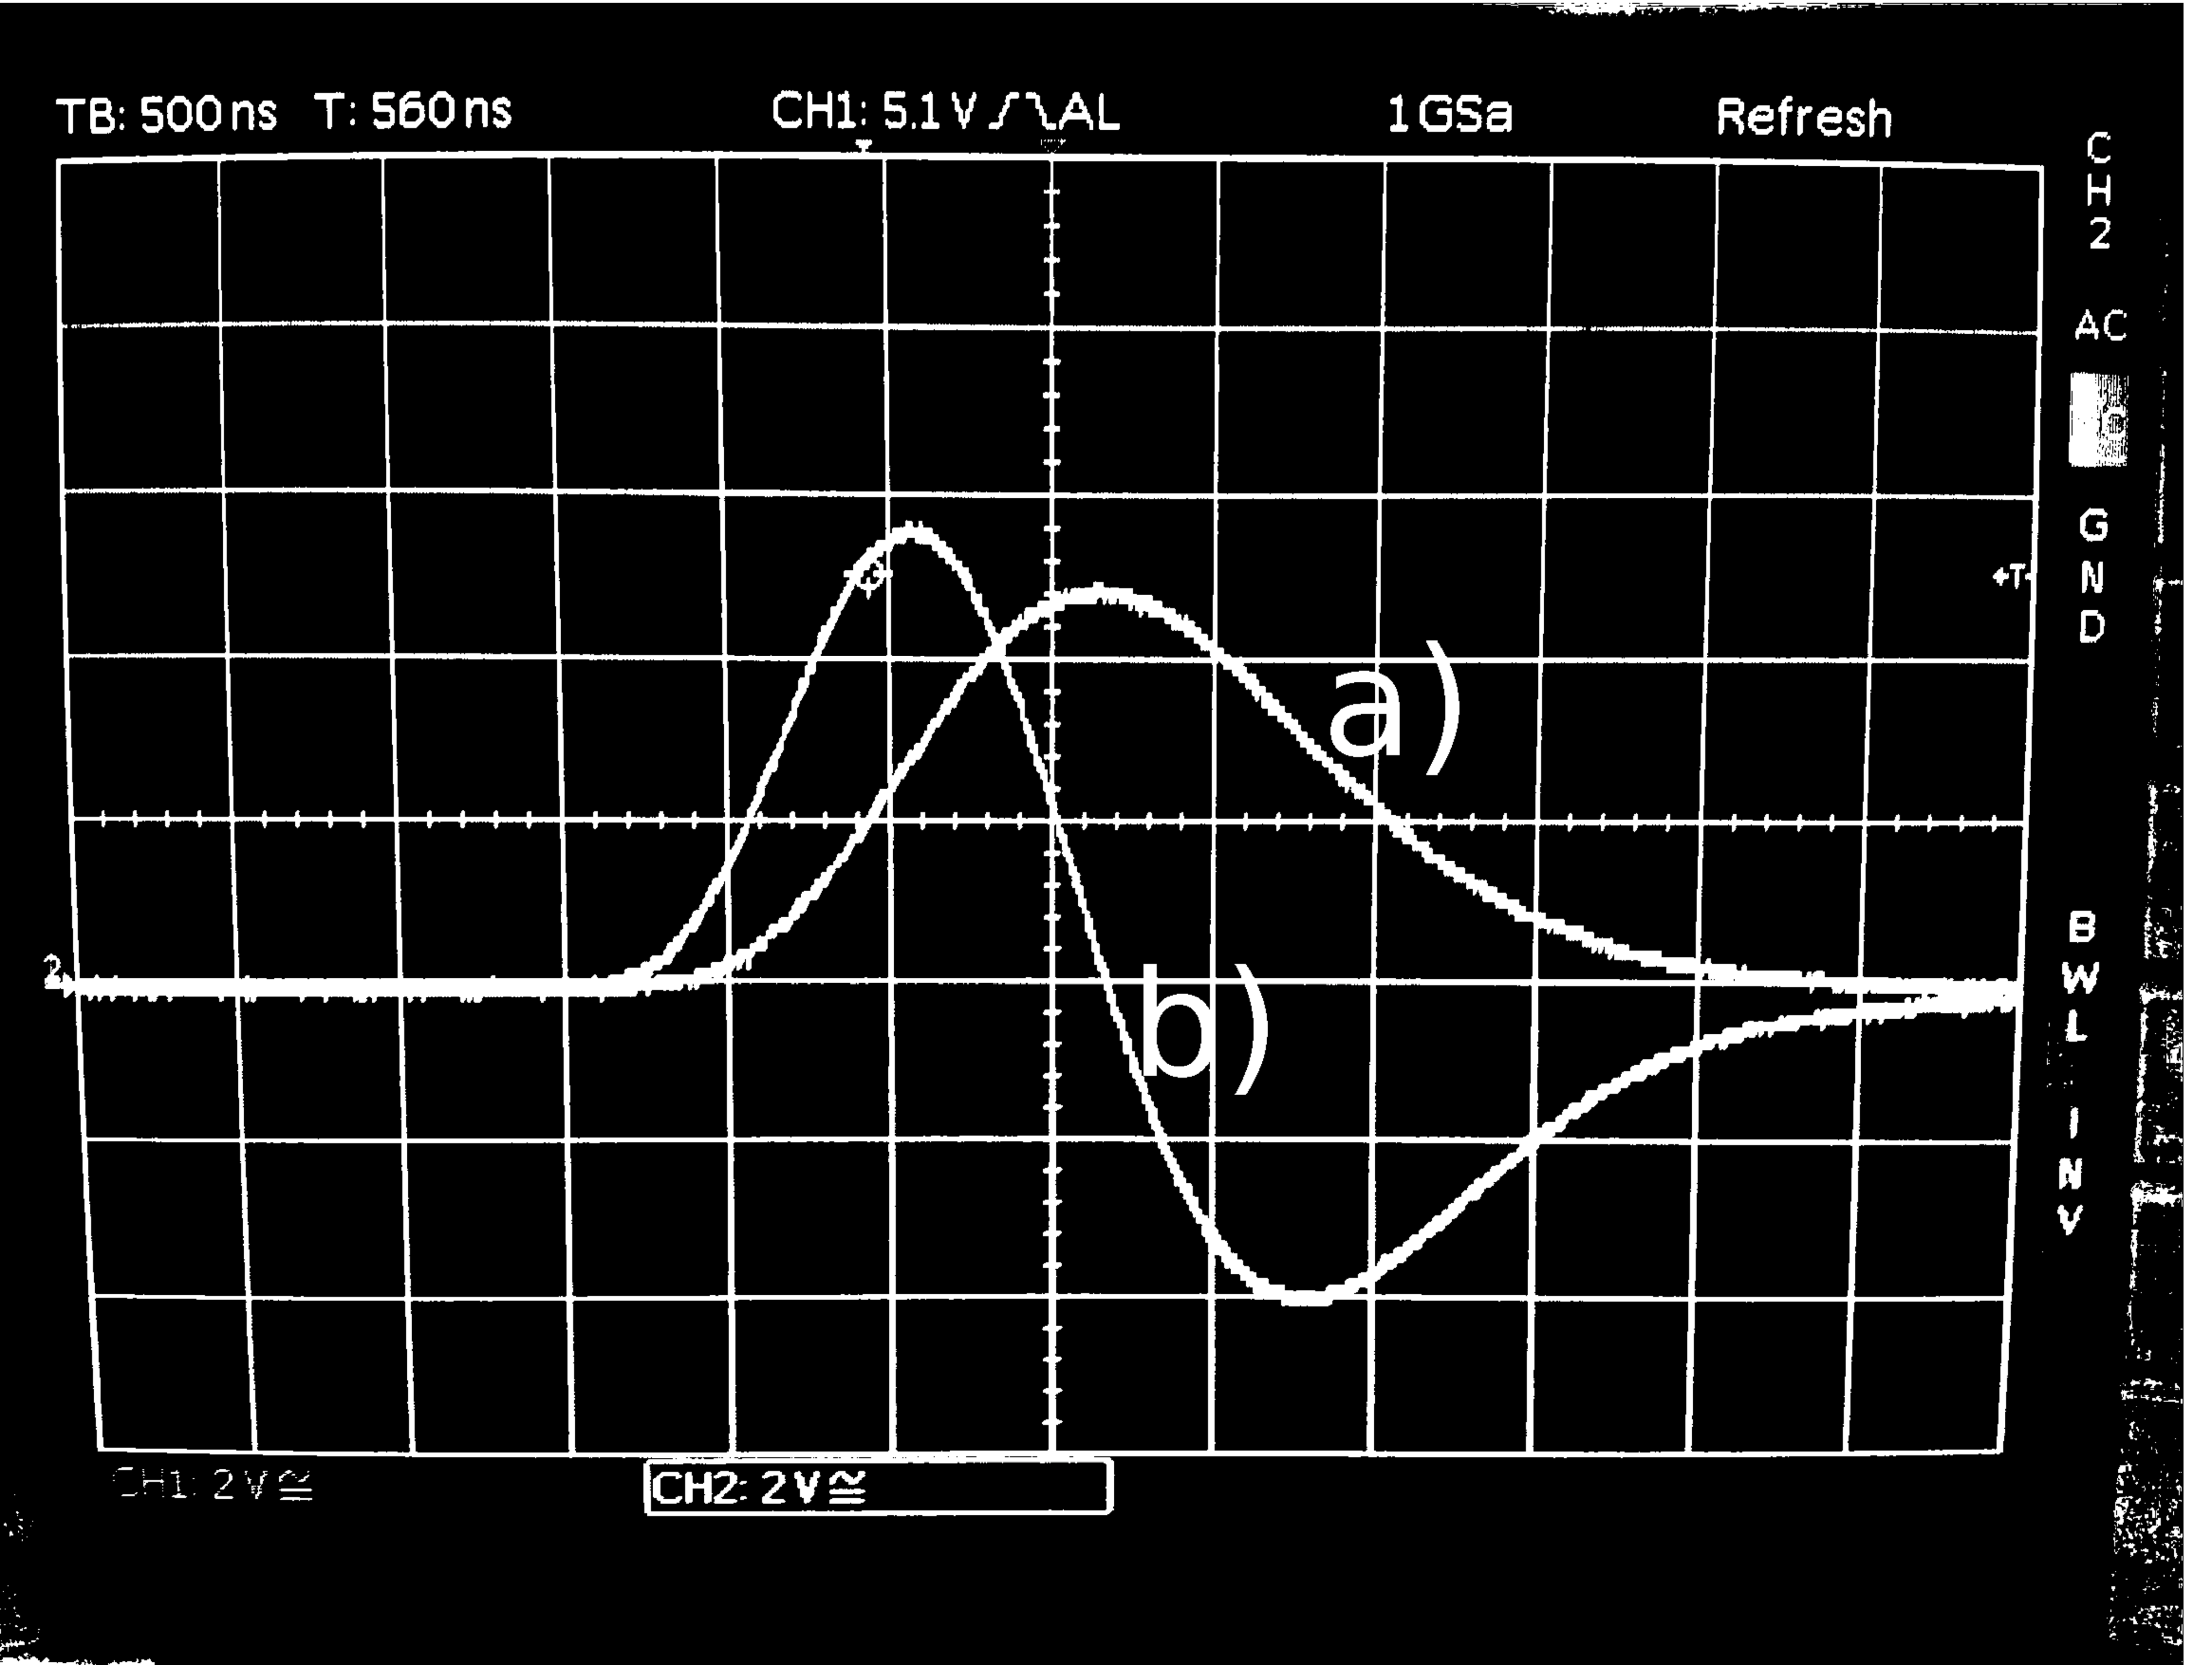
\includegraphics[width=0.8\linewidth]{figures/uni_bipolar2}
    \captionof{figure}{Oscillscope: a) refers to the unipolar channel and b) to 
the bipolar channel.}
  \end{minipage}
  \hfill
  \begin{minipage}[b]{0.49\textwidth}
    \centering
 \begin{tabular}{|l|l|}
     \hline
    course grain & 100\\
    gain    &   10.0 \\
    sharpening time &   0.5 \\
    sample & position 1\\
    PM & Right Side\\
    output & unipolar MCA\\
           & bipolar delay\\
     BLR & AFJ \\
     +/- & Pos \\
     delay & out\\
     \hline
\end{tabular}
\label{tab:config}
  \captionof{table}{Configuration of MA, MCA in measurement 2.1.1.}
    \end{minipage}
\end{minipage}

\subsubsection{Measuring the full energy spectrum}
\label{ssub:Measuring the full energy spectrum}
We increased the gain to 8.6 and the coarse gain to 200 of the MA, such that a observed spectrum 
was distributed of the entire range of bins, in order to be able to decide which detector and position would
be suitable. See Table~\ref{tab:config2} for our configuration of the setup. See
Figure~\ref{fig:measure2.1} for the figures of the measurement 2.1.
\begin{table}[htp]
    \begin{tabular}{|l|l|l||l|l|l|}
        \hline
        2.1a) & Positions:  & Pos1         & 2.1b) & Positions:  & Pos1\\
              & PM          & right        &       & PM          & left \\
              & Time        & $360\pm1$sec &       & Time        & $380\pm1$sec \\
        \hline 
        2.1c) & Positions:  & Pos2         & 2.1d) & Positions:  & Pos2         \\
              & PM          & right        &       & PM          & left \\
              & Time        & $402\pm1$sec &       & Time        & $368\pm1$sec \\
        \hline 
        2.1e) & Positions:  & Pos2         \\
              & PM          & left \\
              & Time        & $360\pm1$sec \\
    \cline{1-3}
    \end{tabular}
  \caption{Configuration in measurement 2.1 of Position, PM and integration time.}
    \label{tab:config2}
\end{table}

\begin{figure}
    \begin{subfigure}[b]{\picwidth}
        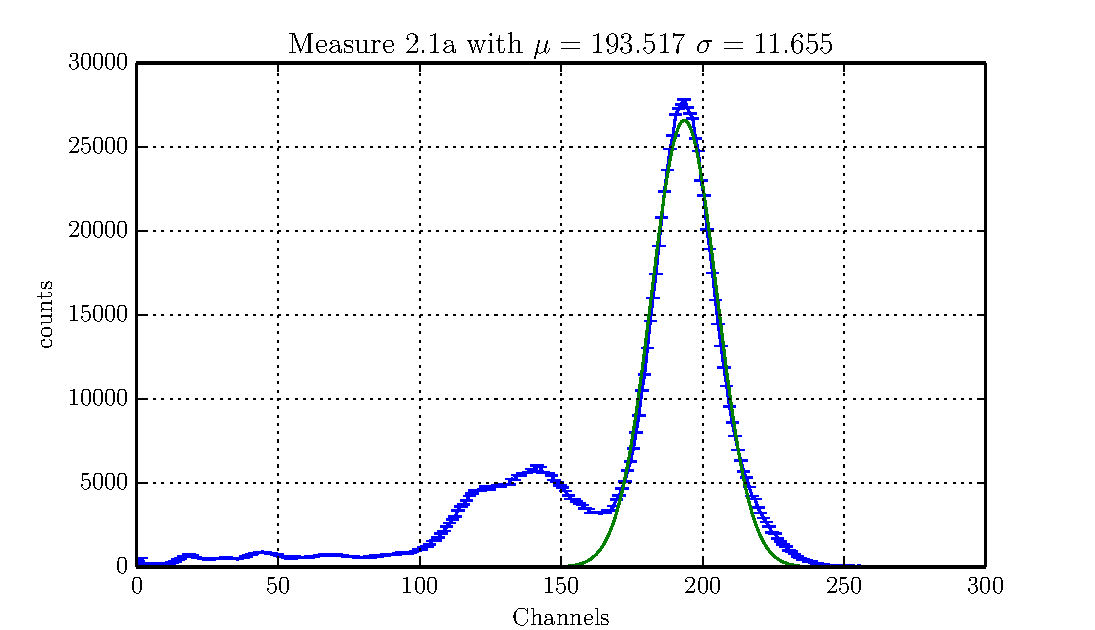
\includegraphics[width=\textwidth]{analysis/figures/plot2_1a}
        \caption{}
    \end{subfigure}\qquad
    \begin{subfigure}[b]{\picwidth}
        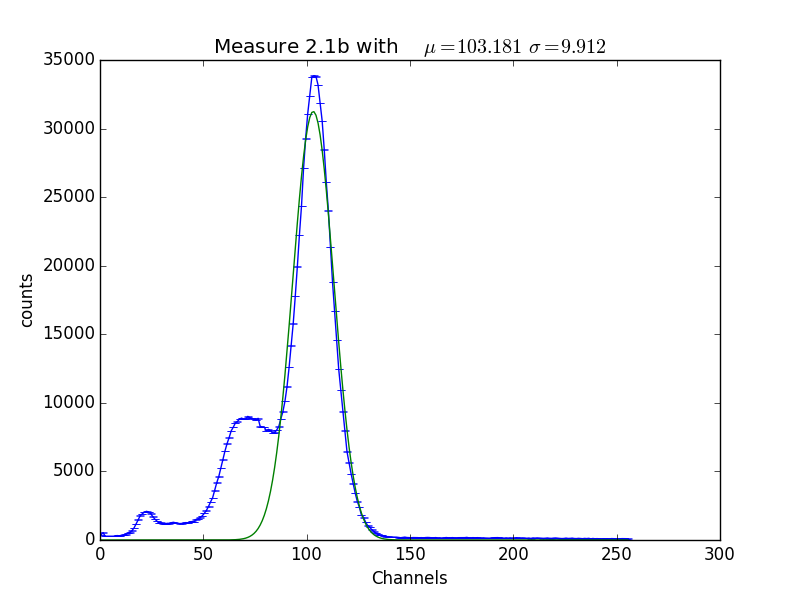
\includegraphics[width=\textwidth]{analysis/figures/plot2_1b}
        \caption{}
    \end{subfigure}
    \begin{subfigure}[b]{\picwidth}
        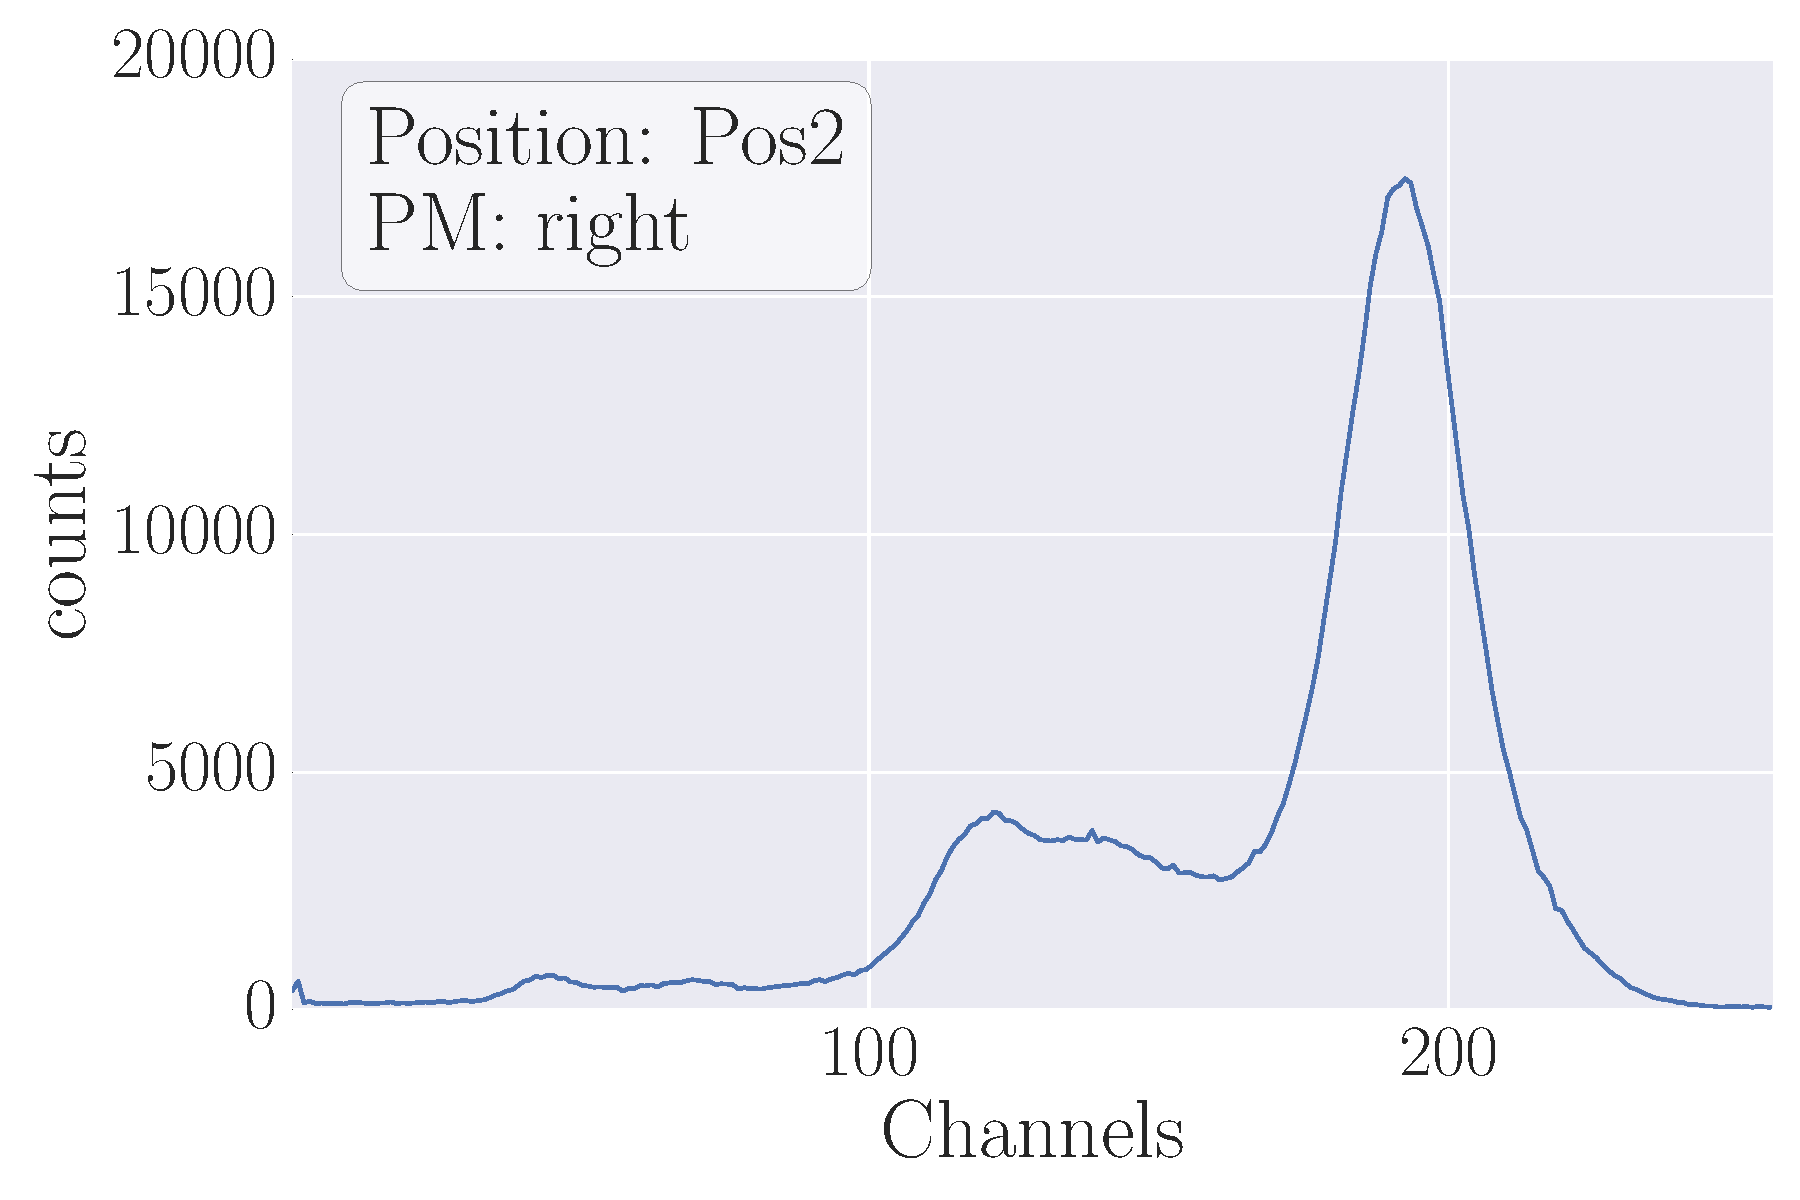
\includegraphics[width=\textwidth]{analysis/figures/plot2_1c}
        \caption{}
    \end{subfigure}
    \begin{subfigure}[b]{\picwidth}
        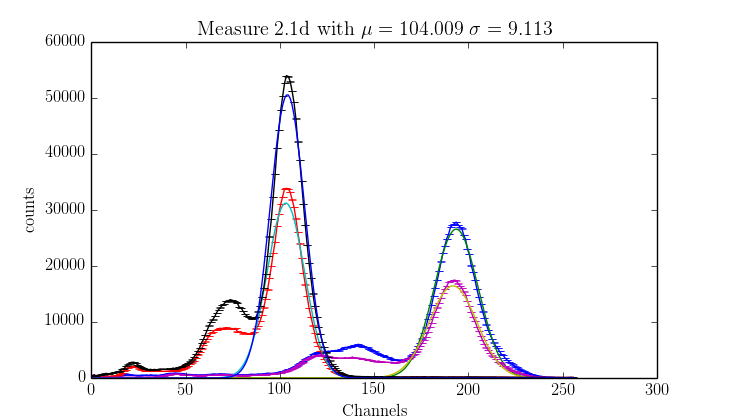
\includegraphics[width=\textwidth]{analysis/figures/plot2_1d}
        \caption{}
    \end{subfigure}
    \begin{subfigure}[b]{\picwidth}
        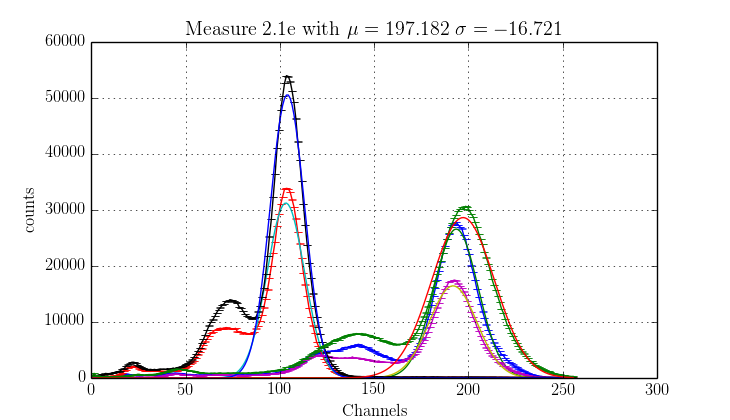
\includegraphics[width=\textwidth]{analysis/figures/plot2_1e}
        \caption{}
    \end{subfigure}
    \caption{Energy spectra with respect to the channels of the MCA, which we prescribed by
        measurements 2.1 (a) - (e).}
    \label{fig:measure2.1}
\end{figure}
\clearpage
\subsection{Measuring $\Delta t$ of coincidences}
\label{sub:measuring_delayed_coincidences}
\subsubsection{Setting the energy window}
\label{ssub:Setting the energy window}
From the results of the last chapter we have decided to chose position 1, which refers to measurements 2.1 a)
and 2.1 b). We only show the configuration of the successfull run with the right energy window chosen.
For the other configurations please see the appended records. For the the time delay we chose
$\Delta t = 140$ns.\\\\ 
 \begin{minipage}{\textwidth}
  \begin{minipage}[b]{0.49\textwidth}
   \begin{tabular}{|l|l|}
        \hline
       14.4 keV signal & right detector \\
       122 keV signal & left detector \\
       coarse gain & 200 \\
       gain & 8.6 \\
       Shaping time & $0.5\mu$s \\
        \hline
   \end{tabular}

  \captionof{table}{Configuration of MA1}
  \end{minipage}
  \hfill
  \begin{minipage}[b]{0.49\textwidth}
    \centering
   \begin{tabular}{|l|l|}
        \hline
       Lower Level & $4.75\pm0.05$ \\
       Upper Level & $3.72\pm0.05$ \\
       Delay & 1.0 (minimum possible) \\
        walk ADJ & $0.1 - 1.1\mu$s (NOR)  \\
       Pos Out & Linear Gate ``enable''\\
        \hline
   \end{tabular}
  \captionof{table}{Configuration of SCA1}
\end{minipage}
\end{minipage}
\begin{minipage}{\textwidth}
  \begin{minipage}[b]{0.49\textwidth}
   \begin{tabular}{|l|l|}
        \hline
       coarse gain & 500 \\
       gain & 8.6 \\
       Shaping time & $0.5\mu$s \\
       input & right detector \\ 
        delay & out \\
        \hline
   \end{tabular}

  \captionof{table}{Configuration of MA2}
  \end{minipage}
  \hfill
  \begin{minipage}[b]{0.49\textwidth}
    \centering
   \begin{tabular}{|l|l|}
        \hline
       Lower Level & $2.02\pm0.05$ \\
       Upper Level & $3.04\pm0.05$ \\
       Delay & 1.0 (minimum possible) \\
        walk ADJ & $0.1 - 1.1\mu$s (NOR)  \\
       Pos Out & Linear Gate ``enable''\\
        \hline
   \end{tabular}
  \captionof{table}{Configuration of SCA2}
\end{minipage}
\end{minipage}
\clearpage
\subsubsection{Delayed coincidences}
The measurement ran about 14 hours over night. See Figure~\ref{fig:4_1} for the visualization.
\label{ssub:Conduction of the experiment over night}

\begin{figure}[htpb]
    \centering
    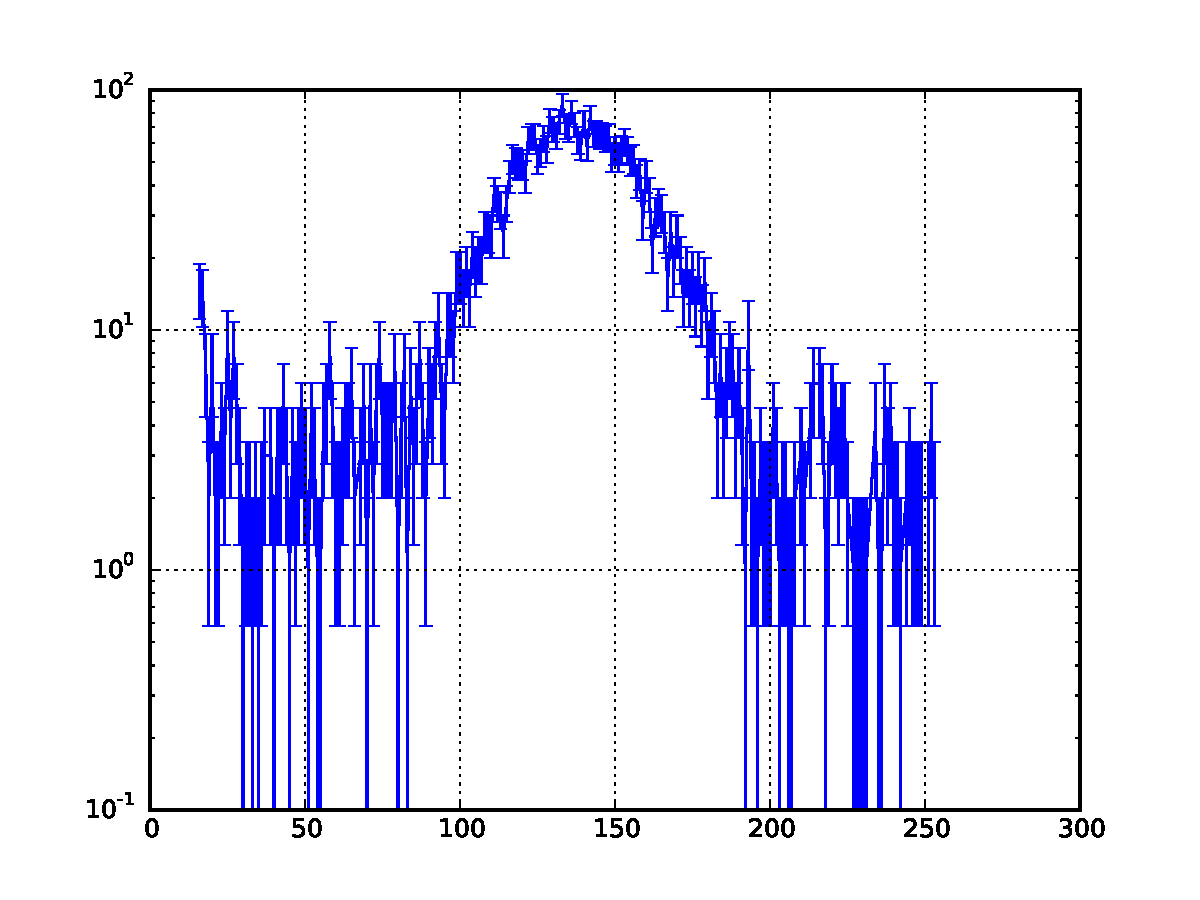
\includegraphics[width=1.0\linewidth]{analysis/figures/plot4_1}
    \caption{Measurement 4.1: You will notice that the shape
        of the peak looks gaussian, which is rather unexpected. However
        further analysis show, that the peak is not symmetric and hence the left 
        side will be fitted against a exponential curve, while the origin of the
        right side is the background, which will be analyzed in the next section.
        The errors which are visualized here are approximated by $S_{N_i} = \sqrt{N_i}$.}
    \label{fig:4_1}
\end{figure}
\clearpage
\subsubsection{Random coicidences}
\label{ssub:Random coicidences}
For measuring the background we used the same configuration as before, except of the TAC-input:
\begin{itemize}
    \item TAC Start: SCA2, triggered by the 14.4 keV Peak, delayed with $\Delta t = 48$ns
    \item TAC Stop: SCA1, triggered by 122 keV (no delay)
\end{itemize}
A first approach with $\Delta t = 16$ns failed, since we observed a clear peak in low channels in contrary
to an expected equally distributed signal. After changing to $\Delta t=48$ns we observe a clear
background noise signal, which you can see in Figure~\ref{fig:5_1}.
\begin{figure}[htpb]
    \centering
    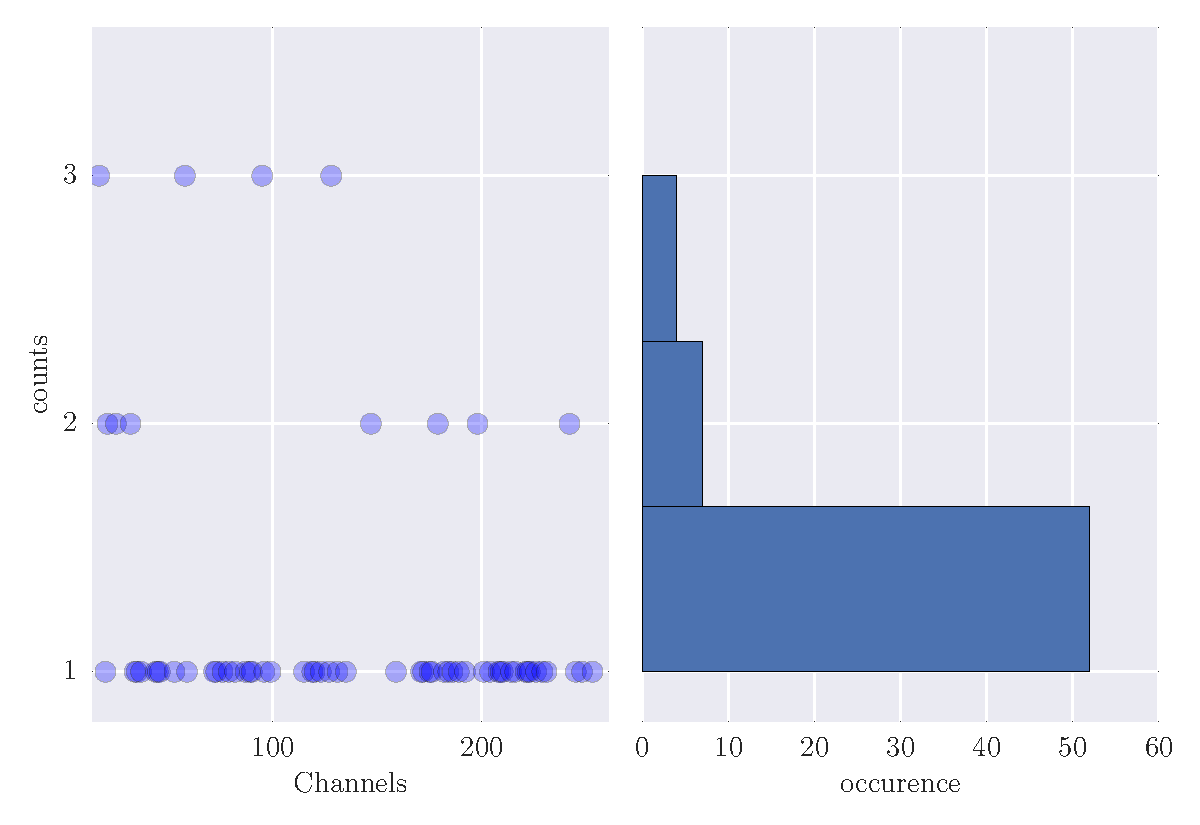
\includegraphics[width=1.0\linewidth]{analysis/figures/plot5_1_hist}
    \caption{Measurement 5.1: Random coincidences and their histogram.}
    \label{fig:5_1}
\end{figure}

\clearpage
\subsection{Calibration of TAC-MCA Signal}
\label{sub:calibration_of_tac_mca_signal}
\begin{figure}[htpb]
    \centering
    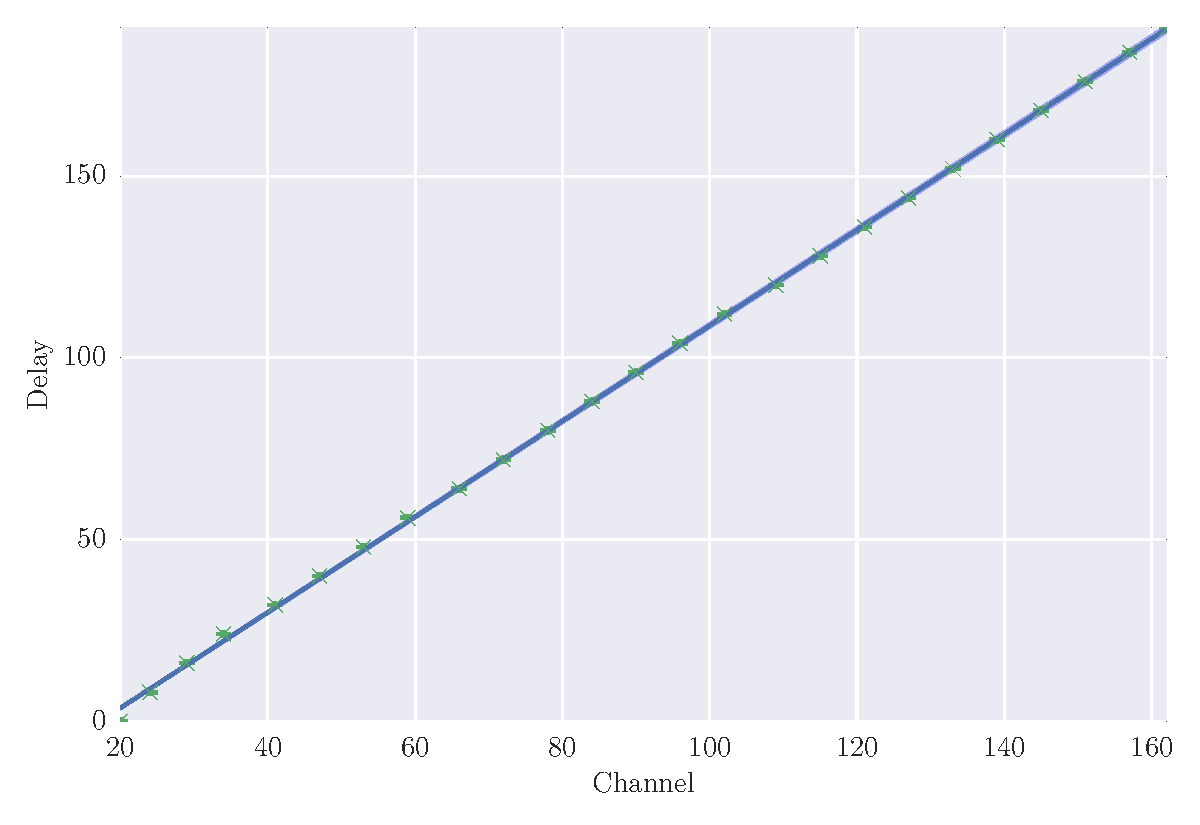
\includegraphics[width=0.7\linewidth]{analysis/figures/plot7}
    \caption{Calibration of the TAC-MCA Signal.}
    \label{fig:plot7}
\end{figure}
\begin{figure}[htpb]
    \centering
    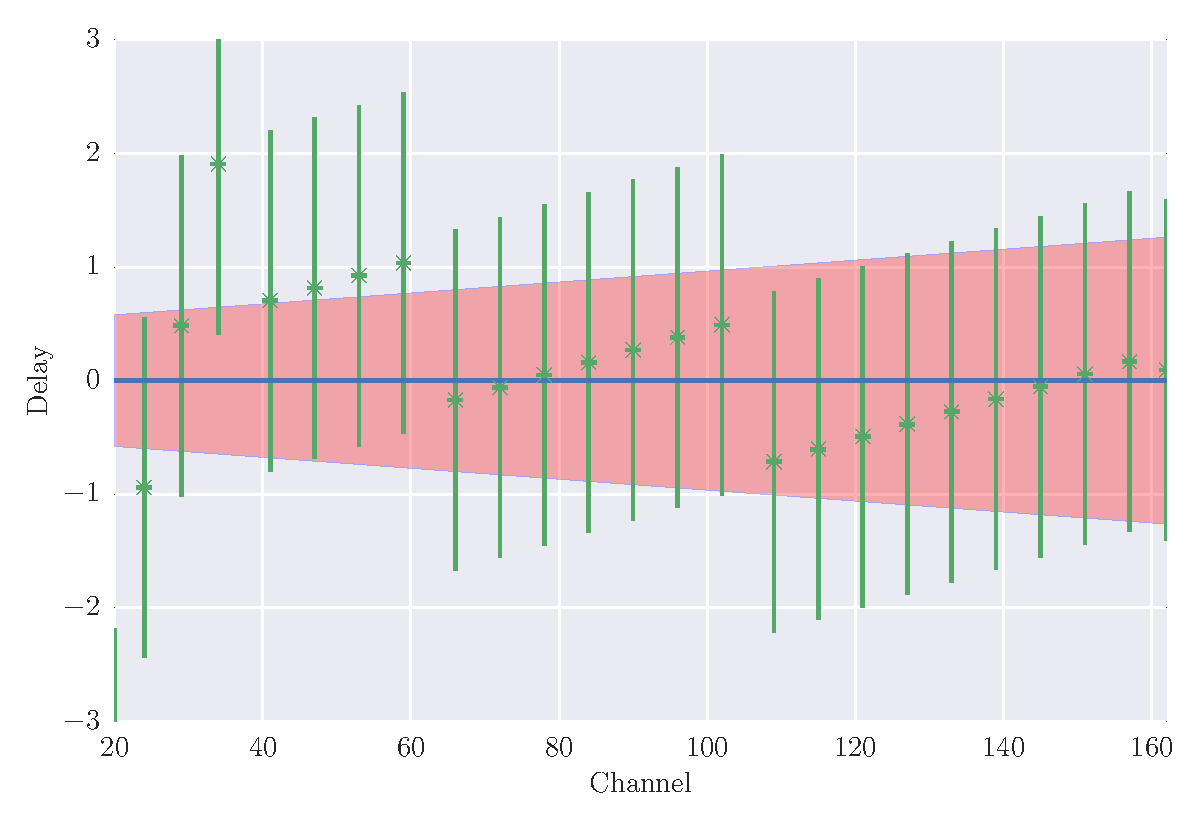
\includegraphics[width=0.7\linewidth]{analysis/figures/plot7b}
    \caption{Calibration of the TAC-MCA Signal.}
    \label{fig:plot7}
\end{figure}




\clearpage

\section{Bibliography}
\printbibliography[heading=subbibintoc]
\clearpage

\end{document}
